\documentclass[a4paper,12pt]{article} 

%%% Работа с русским языком
\usepackage{cmap}					% поиск в PDF
\usepackage{mathtext} 				% русские буквы в фомулах
\usepackage[T2A]{fontenc}			% кодировка
\usepackage[utf8]{inputenc}			% кодировка исходного текста
\usepackage[english,russian]{babel}	% локализация и переносы

%%% Дополнительная работа с математикой
\usepackage{amsmath,amsfonts,amssymb,amsthm,mathtools, gensymb} % AMS
\usepackage{icomma} % "Умная" запятая: $0,2$    ф--- число, $0, 2$ --- перечисление

%%Таблица
\usepackage[table,xcdraw]{xcolor}
\usepackage{caption}
\usepackage{floatrow}
\floatsetup[table]{capposition=top}
\floatsetup[wrapfigure]{capposition=bottom}
\usepackage{multirow}

%Отступы и поля 
\textwidth=18cm
\oddsidemargin=-1cm
\topmargin=-2cm
\textheight=25cm


%% Номера формул
\mathtoolsset{showonlyrefs=true} % Показывать номера только у тех формул, на которые есть \eqref{} в тексте.

%% Шрифты
\usepackage{euscript}	 % Шрифт Евклид
\usepackage{mathrsfs} % Красивый матшрифт

%% Свои команды
\DeclareMathOperator{\sgn}{\mathop{sgn}}

%% Перенос знаков в формулах (по Львовскому)
\newcommand*{\hm}[1]{#1\nobreak\discretionary{}
{\hbox{$\mathsurround=0pt #1$}}{}}

%% Стиль страницы
\usepackage{fancyhdr}

%% Для рисунков
\usepackage{graphicx}
\usepackage[export]{adjustbox}
\usepackage{float}
\usepackage{ragged2e}
\usepackage{wrapfig}

\pagestyle{fancy}
\begin{document}
\begin{titlepage}
\begin{center}
%\vspace*{1cm}
\large{\small ФЕДЕРАЛЬНОЕ ГОСУДАРСТВЕННОЕ АВТОНОМНОЕ ОБРАЗОВАТЕЛЬНОЕ\\ УЧРЕЖДЕНИЕ ВЫСШЕГО ОБРАЗОВАНИЯ \\ МОСКОВСКИЙ ФИЗИКО-ТЕХНИЧЕСКИЙ ИНСТИТУТ\\ (НАЦИОНАЛЬНЫЙ ИССЛЕДОВАТЕЛЬСКИЙ УНИВЕРСИТЕТ)\\ ФАКУЛЬТЕТ АЭРОКОСМИЧЕСКИХ ТЕХНОЛОГИЙ}
\vfill
\line(1,0){490}\\[1mm]
\huge{Лабораторная работа 4.4.1}\\
\huge\textbf{Изучение амплитудной дифракционной решётки}\\
\line(1,0){490}\\[1mm]
\vfill
\begin{flushright}
\normalsize{Рогозин Владимир}\\
\normalsize{\textbf{Группа Б03-106}}\\
\end{flushright}
\end{center}
\end{titlepage}
\fancyhead[L] {Работа 4.4.1}

\textbf{Цель работы}: 
Знакомство с работой и настройкой гониометра Г5, определение спектральных характеристик амплитудной решётки.

\textbf{Оборудование}:
Гониометр, дифракционная решётка, ртутная лампа.

\textbf{Теоретические сведения}:

\textbf{Амплитудная дифракционная решётка.} Амплитудную решётку можно представить в виде непрозрачного экрана, в котором прорезано большое число $N$ параллельных щелей -- штрихов. Постоянство расстояний между штрихами $d$ -- \textit{периодом} решётки, и шириной штриха $b$ должно выдерживаться с большой точностью. 

\begin{wrapfigure}[21]{l}{0.4\textwidth}\label{fig: Amplitude grating}
    \begin{center}
    \vspace{-20pt}
        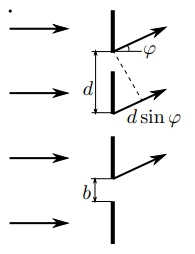
\includegraphics[width = 0.75\textwidth]{Amplitude grating.png}
    \end{center}
    \caption{ Дифракция световой волны на амплитудной решётке}
\end{wrapfigure}

Наблюдение изображения спектра проводится с помощью зрительной трубы, настроенной на бесконечность (дифракция Фраунгофера на штрихах решётки). В этом случае амплитуда и интенсивность поля световой волны определяются углом $\varphi$ между нормалью к решётке и направлением дифрагировавших лучей. 

Пусть падающая на решётку волна распространяется перпендикулярно её поверхности. Интенсивность дифрагированного света максимальна для углов $\varphi_m$, для которых волны, приходящие в точку наблюдения от всех щелей решётки, оказываются в фазе:
\begin{equation}\label{eq: max condition}
    d \sin{\varphi_m} = m \lambda.
\end{equation}
Величина $m = 0, \pm 1, \pm 2, ...$ называется порядком спектра.

Точная теория решётки учитывает как интерференцию волн, приходящих от разных щелей, так и дифракцию на каждой щели. Как показывает простой расчёт, интенсивность $I$ света, распространяющегося под углом $\varphi$ к нормали, определяется формулой
\begin{equation}\label{eq: intensity via phi}
    I = I_1(\varphi) \frac{\sin^2[N(kd \sin\varphi) / 2]}{\sin^2[(kd \sin\varphi) / 2]},
\end{equation}
где $k = 2\pi / \lambda$ -- волновое число, а множитель $I_1(\varphi)$ описывает дифракцию волн, испускаемых одним периодом решётки (\textit{диаграмма направленности} одного периода).

Анализ выражения \eqref{eq: intensity via phi} показывает, что при большом числе щелей свет, прошедший через решётку, распространяется по ряду резко ограниченных направлений, определяемых соотношением \eqref{eq: max condition}. 

\begin{wrapfigure}[13]{l}{0.4\textwidth}\label{fig: Intensity distribution}
    \begin{center}
    \vspace{-20pt}
        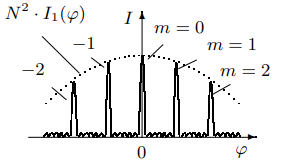
\includegraphics[width = 0.9\textwidth]{Intensity distribution.png}
    \end{center}
    \caption{Распределение интенсивности света при дифракции Фраунгофера на решётке}
\end{wrapfigure}
Зависимость интенсивности света от угла наблюдения представлена на рис. 2.

Как следует из \eqref{eq: max condition}, углы, при которых наблюдаются световые максимумы, зависят от длины волны $\lambda$. Дифракционная решётка представляет собой, таким образом, \textit{спектральный прибор}. Если на дифракционную решётку падает свет сложного спектрального состава, то после решётки образуется спектр, причём фиолетовые лучи отклоняются решёткой меньше, чем красные. При $m = 0$ максимумы интенсивности для всех длин волн располагаются при $\varphi = 0$ и накладываются друг на друга. При освещении белым светом нулевой максимум, в отличие от всех прочих, оказывается поэтому неокрашенным. Спектры первого, второго и т. д. порядков располагаются симметрично по обе стороны от нулевого.

\textbf{Угловая дисперсия.} Дисперсия $D$ характеризует угловое расстояние между близкими спектральными линиями:
\begin{equation}\label{eq: angle dispersion}
    D = \frac{d\varphi}{d\lambda}.
\end{equation}
По величине \textit{угловой дисперсии} можно определить угловое расстояние между двумя близкими спектральными линиями: $\delta \varphi \approx \delta \lambda$.

Дифференцируя обе части \eqref{eq: max condition} получим
\[d \cdot \cos\varphi d\varphi = m \cdot d\lambda.\]
Следовательно, 
\[D = \frac{d\varphi}{d\lambda} = \frac{m}{d \cos\varphi} = \frac{m}{\sqrt{d^2 - m^2 \lambda^2}}.\]

Дисперсия возрастает с увеличением порядка спектра. На опыте дисперсию решётки определяют путём измерения углового расстояния $\Delta\varphi$
между двумя близкими спектральными линиями с известной разностью длин волн $\Delta\lambda$ (например, между жёлтыми линиями ртути).

\textbf{Разрешающая способность дифракционной решётки.} $R = \lambda / \delta\lambda$ характеризует возможность прибора различать две близкие спектральные линии с длинами волн $\lambda$ и $\lambda + \delta\lambda$. Возможность разрешения двух близких спектральных линий зависит от их ширины и от расстояния между ними. 

Пусть в спектре $m$-го порядка наблюдаются две близкие спектральные линии с длинами волн $\lambda$ и ($\lambda + \Delta\lambda$). Угловое расстояние
$\Delta\varphi$ между этими линиями равно
\[\Delta\varphi = \frac{m \Delta\lambda}{d\cos\varphi}.\]

\begin{wrapfigure}[22]{r}{0.5\textwidth}\label{fig: Rayleigh's criterion}
    \begin{center}
    \vspace{-20pt}
        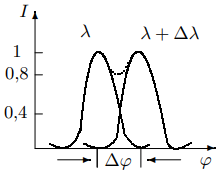
\includegraphics[width = 0.9\textwidth]{Rayleigh's criterion.png}
    \end{center}
    \caption{К определению разрешающей способности дифракционной решётки}
\end{wrapfigure}
Согласно \textit{критерию разрешения Релея} линии становятся неразличимыми, когда расстояние между ними меньше, чем расстояние от максимума одной линии до её первого минимума. Как следует из \eqref{eq: intensity via phi}, при переходе из главного максимума ($\varphi = 0$) в минимум величина $ N(kd\sin\varphi) / 2$ изменяется на $\pi$, так что
\[\frac{Nkd}{2}[\sin(\varphi + \delta\varphi) - \sin(\varphi)] = \pi,\]
где $\delta\varphi$ -- угловая полуширина главного максимума. Принимая во внимание малость $\delta\varphi$, получим
\[\delta\varphi = \frac{\lambda}{Nd\cos\varphi}.\]

Приравнивая $\delta\varphi$ и $\Delta\varphi$ для случая предельного разрешения, найдём для \textit{разрешающую способность} дифракционной решётки
\begin{equation}
    R = \frac{\lambda}{\delta\lambda} = m \cdot N.
\end{equation}


\textbf{Дисперсионная область.} При достаточно широком спектральном интервале падающего света спектры разных порядков могут накладываться друг на друга. Предельная ширина спектрального интервала $\Delta\lambda$, при которой спектры соседних порядков ($m$ и $m + 1$) перекрываются только своими границами, называется \textit{дисперсионной областью} $G$. При этом 
\[d\sin\varphi = m(\lambda + \Delta\lambda ) = (m + 1)\lambda,\]
и дисперсионная область
\begin{equation}\label{eq: dispersion region}
    G = \Delta\lambda = \frac{\lambda}{m}.
\end{equation}

\textbf{Экспериментальная установка}:

При работе с дифракционной решёткой основной задачей является точное измерение углов, при которых наблюдаются главные максимумы для различных длин волн. В этой работе для измерения углов используется гониометр Г5. Принципиальная схема экспериментальной установки приведена на рис. 4.

\begin{wrapfigure}[10]{r}{0.5\textwidth}\label{fig: Experimental setup}
    \begin{center}
    \vspace{-20pt}
        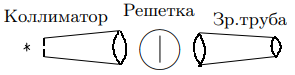
\includegraphics[width = 0.9\textwidth]{Experimental setup.png}
    \end{center}
    \caption{Схема экспериментальной установки (вид сверху)}
\end{wrapfigure}    
\textbf{Измерение длин волн спектральных линий.} Дифракционная решётка
с известным периодом может быть использована для измерения длин волн, например, в спектре ртути. Как следует из \eqref{eq: max condition}, измерения длины волны сводятся к определению $\varphi_m$ -- угла отклонения лучей от первоначального направления. Проведя измерения дифракционных углов для спектра с известными длинами волн, можно рассчитать период решётки.

\textbf{Определение угловой дисперсии.} Для определения угловой дисперсии
дифракционной решётки нужно измерить угловое расстояние $\Delta\varphi$ между двумя близкими спектральными линиями с длинами волн $\lambda_1$ и $\lambda_2$ и провести вычисления по формуле $D = \Delta\varphi / (\lambda_1 - \lambda_2)$.

\textbf{Оценка разрешающей способности решётки.} Непосредственное экспериментальное определение разрешающей способности дифракционной решётки требует специальных источников света, в спектре которых имеются близкие спектральные линии, находящиеся на пределе разрешения. Обозначим через $\delta\lambda$ разность их длин волн. Разрешающая сила определяется отношением $\lambda / \delta\lambda$.

\textbf{Обработка данных}:  
\begin{enumerate}
    \item Сначала, с помощью стеклянной призмы, проведём юстировку гониометра и установим начало отсчёта, запишем характеристики спектра ртутной лампы.  
    \begin{table}[H]\label{Hg lamp spectrum}
        \centering
        \begin{tabular}{|
            >{\columncolor[HTML]{FFFFFF}}c |
            >{\columncolor[HTML]{FFFFFF}}c |
            >{\columncolor[HTML]{FFFFFF}}c |
            >{\columncolor[HTML]{FFFFFF}}c |
            >{\columncolor[HTML]{FFFFFF}}c |
            >{\columncolor[HTML]{FFFFFF}}c |
            >{\columncolor[HTML]{FFFFFF}}c |
            >{\columncolor[HTML]{FFFFFF}}c |
            >{\columncolor[HTML]{FFFFFF}}c |}
            \hline
            {\color[HTML]{000000} Цвет} &
              {\color[HTML]{000000} красн.} &
              {\color[HTML]{000000} красн.} &
              {\color[HTML]{000000} желт.} &
              {\color[HTML]{000000} желт.} &
              {\color[HTML]{000000} зелен.} &
              {\color[HTML]{000000} голуб.} &
              {\color[HTML]{000000} синий} &
              {\color[HTML]{000000} фиолет.} \\ \hline
            {\color[HTML]{000000} $\lambda$, нм} &
              {\color[HTML]{000000} 690,7} &
              {\color[HTML]{000000} 623,4} &
              {\color[HTML]{000000} 579,1} &
              {\color[HTML]{000000} 577,0} &
              {\color[HTML]{000000} 546,1} &
              {\color[HTML]{000000} 491,6} &
              {\color[HTML]{000000} 435,8} &
              {\color[HTML]{000000} 404,7} \\ \hline
        \end{tabular}
        \caption{Характеристики спектра ртутной лампы ДРШ}
    \end{table}

    \item Далее, убедимся в справедливости формулы \eqref{eq: max condition}, для этого запишем значение периода решётки $d = 1 / 500 \text{ мм} = 2 \text{ мкм}$, затем определим углы дифракции для двух ярких линий спектра в одном порядке и убедимся, что $d \sin\varphi \sim \lambda$. 
    \begin{table}[H]\label{tab: max cond estimation }
        \centering
        \begin{tabular}{|
            >{\columncolor[HTML]{FFFFFF}}c |
            >{\columncolor[HTML]{FFFFFF}}c |
            >{\columncolor[HTML]{FFFFFF}}c |
            >{\columncolor[HTML]{FFFFFF}}c |}
            \hline
            {\color[HTML]{000000} Цвет} &
              {\color[HTML]{000000} $\varphi$} &
              {\color[HTML]{000000} $\lambda_{эксп.}$, нм} &
              {\color[HTML]{000000} $\lambda_{табл.}$, нм} \\ \hline
            {\color[HTML]{000000} Синий} &
              {\color[HTML]{000000} $12\degree 35'57''$} &
              {\color[HTML]{000000} 436,3} &
              {\color[HTML]{000000} 435,8} \\ \hline
            {\color[HTML]{000000} Голубой} &
              \cellcolor[HTML]{FFFFFF}{\color[HTML]{000000} $14\degree 15'57''$} &
              {\color[HTML]{000000} 492,8} &
              {\color[HTML]{000000} 491,6} \\ \hline
        \end{tabular}
        \caption{Результаты оценки формулы \eqref{eq: max condition}}
    \end{table}

    \item Теперь будем измерять угловые координаты спектральных линий ртути в $\pm 1$ порядках. Результаты измерений приведены в таблице ниже.
    \begin{table}[H]\label{tab: 1 and -1 order data}
        \centering
        \begin{tabular}{|
            >{\columncolor[HTML]{FFFFFF}}c |
            >{\columncolor[HTML]{FFFFFF}}c |
            >{\columncolor[HTML]{FFFFFF}}c |}
            \hline
            {\color[HTML]{000000} }        & {\color[HTML]{000000} $m = 1$}            & \cellcolor[HTML]{FFFFFF}{\color[HTML]{000000} $m = -1$} \\ \hline
            {\color[HTML]{000000} Цвет}    & {\color[HTML]{000000} $\varphi$}          & {\color[HTML]{000000} $\varphi$}                        \\ \hline
            {\color[HTML]{000000} Фиолетовый} & {\color[HTML]{000000} $12\degree 48'25''$}                         & {\color[HTML]{000000} $12\degree 41'58''$} \\ \hline
            {\color[HTML]{000000} Голубой} & {\color[HTML]{000000} $14\degree 18'9''$} & {\color[HTML]{000000} $14\degree 5'0''$}                   \\ \hline
            {\color[HTML]{000000} Зелёный}    & \cellcolor[HTML]{FFFFFF}{\color[HTML]{000000} $15\degree 46'59''$} & {\color[HTML]{000000} $15\degree 55'1''$}  \\ \hline
            {\color[HTML]{000000} Желтый 1}   & \cellcolor[HTML]{FFFFFF}{\color[HTML]{000000} $16\degree 52'37''$} & {\color[HTML]{000000} $16\degree 50'0''$}     \\ \hline
            {\color[HTML]{000000} Желтый 2}   & \cellcolor[HTML]{FFFFFF}{\color[HTML]{000000} $16\degree 58'1''$}  & {\color[HTML]{000000} $16\degree 57'0''$}     \\ \hline
        \end{tabular}
        \caption{Результаты измерений для $m = \pm 1$ порядков}
    \end{table}
    По результатам измерений построим график зависимости $\sin\varphi$ от $\lambda$ для каждого из порядков, по углу наклона прямой вычислим период дифракционной решетки, сравним полученное значение с истинным. 
    \begin{table}[H]\label{tab: d results}
        \centering
        \begin{tabular}{|
            >{\columncolor[HTML]{FFFFFF}}c |
            >{\columncolor[HTML]{FFFFFF}}c |
            >{\columncolor[HTML]{FFFFFF}}c |
            >{\columncolor[HTML]{FFFFFF}}c |
            >{\columncolor[HTML]{FFFFFF}}c |}
            \hline
            {\color[HTML]{000000} $d$, мкм} &
              {\color[HTML]{000000} $d_1$, мкм} &
              {\color[HTML]{000000} $\varepsilon_{d_1}$, \%} &
              {\color[HTML]{000000} $d_{-1}$, мкм} &
              {\color[HTML]{000000} $\varepsilon_{d_{-1}}$, \%} \\ \hline
            {\color[HTML]{000000} 2,0} &
              {\color[HTML]{000000} 1,98} &
              \cellcolor[HTML]{FFFFFF}{\color[HTML]{000000} 1,24} &
              {\color[HTML]{000000} 1,97} &
              {\color[HTML]{000000} 1,32} \\ \hline
        \end{tabular}
        \caption{Результаты определения периода решётки }
    \end{table}

    \item После этого, определим угловые координаты линий жёлтой пары во всех видимых порядках спектра. Результаты измерений приведены в таблице ниже.
    \begin{table}[H]\label{tab: yellow duplet data}
        \centering
        \begin{tabular}{|
            >{\columncolor[HTML]{FFFFFF}}c |
            >{\columncolor[HTML]{FFFFFF}}c |
            >{\columncolor[HTML]{FFFFFF}}c |
            >{\columncolor[HTML]{FFFFFF}}c |
            >{\columncolor[HTML]{FFFFFF}}c |
            >{\columncolor[HTML]{FFFFFF}}c |}
            \hline
            {\color[HTML]{000000} $m$} &
              {\color[HTML]{000000} Цвет} &
              {\color[HTML]{000000} $\varphi$} &
              {\color[HTML]{000000} $m$} &
              {\color[HTML]{000000} Цвет} &
              {\color[HTML]{000000} $\varphi$} \\ \hline
            \cellcolor[HTML]{FFFFFF}{\color[HTML]{000000} } &
              {\color[HTML]{000000} желт. 1} &
              {\color[HTML]{000000} $16\degree 53'$} &
              \cellcolor[HTML]{FFFFFF}{\color[HTML]{000000} } &
              {\color[HTML]{000000} желт. 1} &
              {\color[HTML]{000000} $16\degree 50'$} \\ \cline{2-3} \cline{5-6} 
            \multirow{-2}{*}{\cellcolor[HTML]{FFFFFF}{\color[HTML]{000000} 1}} &
              {\color[HTML]{000000} желт. 2} &
              {\color[HTML]{000000} $16\degree 58'$} &
              \multirow{-2}{*}{\cellcolor[HTML]{FFFFFF}{\color[HTML]{000000} -1}} &
              {\color[HTML]{000000} желт. 2} &
              {\color[HTML]{000000} $16\degree 57'$} \\ \hline
            \cellcolor[HTML]{FFFFFF}{\color[HTML]{000000} } &
              {\color[HTML]{000000} желт. 1} &
              {\color[HTML]{000000} $34\degree 30'$} &
              \cellcolor[HTML]{FFFFFF}{\color[HTML]{000000} } &
              {\color[HTML]{000000} желт. 1} &
              {\color[HTML]{000000} $34\degree 5'$} \\ \cline{2-3} \cline{5-6} 
            \multirow{-2}{*}{\cellcolor[HTML]{FFFFFF}{\color[HTML]{000000} 2}} &
              {\color[HTML]{000000} желт. 2} &
              {\color[HTML]{000000} $35\degree 38'$} &
              \multirow{-2}{*}{\cellcolor[HTML]{FFFFFF}{\color[HTML]{000000} -2}} &
              {\color[HTML]{000000} желт. 2} &
              {\color[HTML]{000000} $35\degree 10'$} \\ \hline
            \cellcolor[HTML]{FFFFFF}{\color[HTML]{000000} } &
              {\color[HTML]{000000} желт. 1} &
              {\color[HTML]{000000} $61\degree 28'$} &
              \cellcolor[HTML]{FFFFFF}{\color[HTML]{000000} } &
              {\color[HTML]{000000} желт. 1} &
              {\color[HTML]{000000} $58\degree 43'$} \\ \cline{2-3} \cline{5-6} 
            \multirow{-2}{*}{\cellcolor[HTML]{FFFFFF}{\color[HTML]{000000} 3}} &
              {\color[HTML]{000000} желт. 2} &
              {\color[HTML]{000000} $62\degree 7'$} &
              \multirow{-2}{*}{\cellcolor[HTML]{FFFFFF}{\color[HTML]{000000} -3}} &
              {\color[HTML]{000000} желт. 2} &
              {\color[HTML]{000000} $59\degree 4'$} \\ \hline
        \end{tabular}
        \caption{угловые координаты линий жёлтой пары в трёх порядка спектра}
    \end{table}

    \item
    Теперь оценим разрешающую способность решётки. Для этого измерим координату и угловую ширину жёлтой линии.
    \[R = \frac{\varphi}{\delta\varphi}\]
    \begin{table}[H]\label{tab: R result}
        \centering
        \begin{tabular}{|
            >{\columncolor[HTML]{FFFFFF}}c |
            >{\columncolor[HTML]{FFFFFF}}c |
            >{\columncolor[HTML]{FFFFFF}}c |}
            \hline
            {\color[HTML]{000000} $\delta\lambda$} & {\color[HTML]{000000} $\lambda$}       & {\color[HTML]{000000} $R$}      \\ \hline
            {\color[HTML]{000000} $6'$}            & {\color[HTML]{000000} $16\degree 53'$} & {\color[HTML]{000000} 9 608,83} \\ \hline
        \end{tabular}
        \caption{Разрешающая способность решётки}
\end{table}
    
\end{enumerate}


\textbf{Вывод}:
В данной работе было исследовано явления дифракции на амплитудной решётке. С помощью угловых координат 1-го и -1-го порядков спектра был рассчитан и сравнён с истинным значением период дифракционной решётки. Также, была получена и сравнена с теоретической зависимость угловой дисперсии от порядка спектра, и по угловой ширине жёлтой пары была найдена разрешающая способность амплитудной решётки.

%%%%%%%%%%%%%%%%%%%%%%%%% Графики
\newpage
\begin{figure}[H]\label{fig: sin_phi(lambd)}
    \centering
    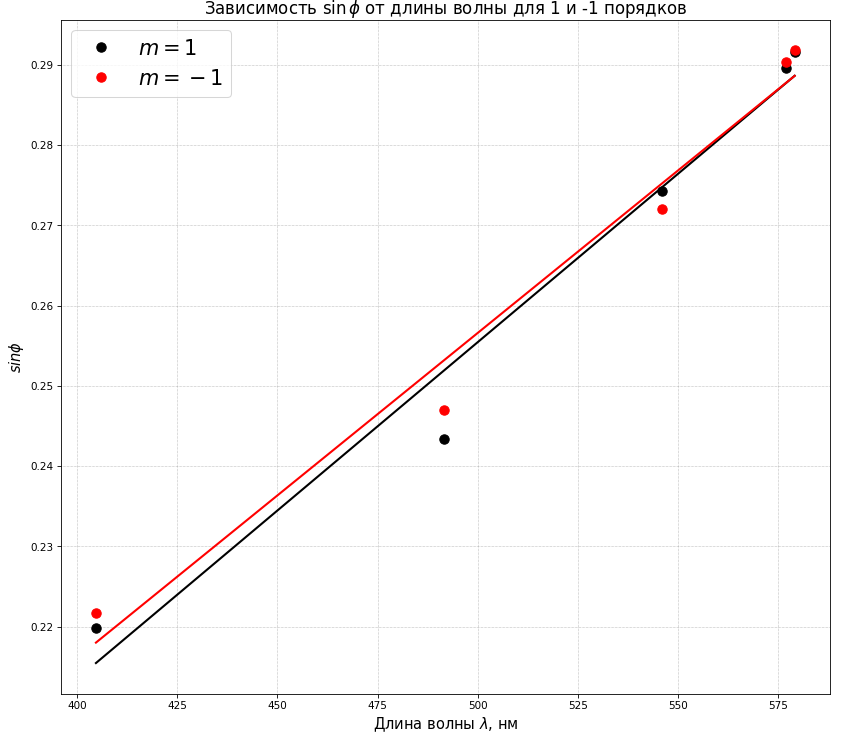
\includegraphics[width = \textwidth]{sin_phi(lambd).png}
\end{figure}
\[k_1 = (506,05 \pm 6,25)\cdot 10^{-6}\text{ }нм^{-1} \quad \varepsilon_{k_1} \approx 1,24\%\]
\[d_1 = (197,61 \pm 2,45)\cdot 10^{-8}\text{ }м \quad \varepsilon_{d_1} \approx 1,24\%\]


\[k_{-1} = (507,45 \pm 6,70)\cdot 10^{-6}\text{ }нм^{-1} \quad \varepsilon_{k_{-1}} \approx 1,32\%\]
\[d_{-1} = (197,06 \pm 2,60)\cdot 10^{-8}\text{ }м \quad \varepsilon_{d_{-1}} \approx 1,32\%\]



\newpage
\begin{figure}[H]\label{fig: D(m)}
    \centering
    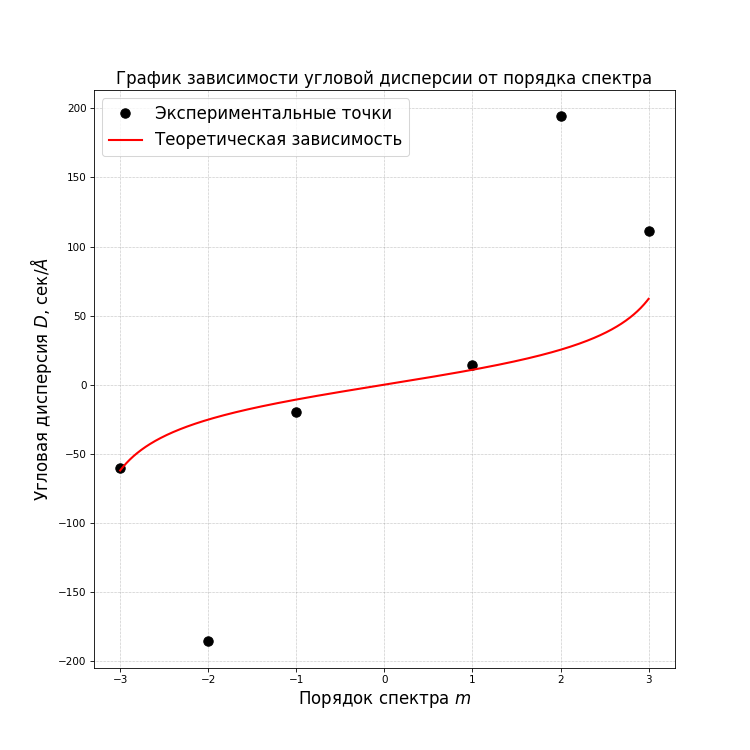
\includegraphics[width = \textwidth]{D(m).png}
\end{figure}


%%%%%%%%%%%%%%%%%%%%%%%%%
\end{document}
